\subsection{The Cherenkov Telescope Array}

\begin{frame}{The Cherenkov Telescope Array (CTA)}
  \begin{minipage}{0.48\textwidth}
    \begin{itemize}
      \setlength\itemsep{1em}
      \item 2 sites: CTA North and CTA South
      \item 3 types of telescopes:
      \begin{itemize}
        \setlength\itemsep{0.5em}
        \item [•] Small-Sized Telescope (SST)
        \item [•] Medium-Sized Telescope (MST)
        \item [•] Large-Sized Telescope (LST)
      \end{itemize}
    \end{itemize}
  \end{minipage}
  \begin{minipage}{0.48\textwidth}
    \begin{center}
      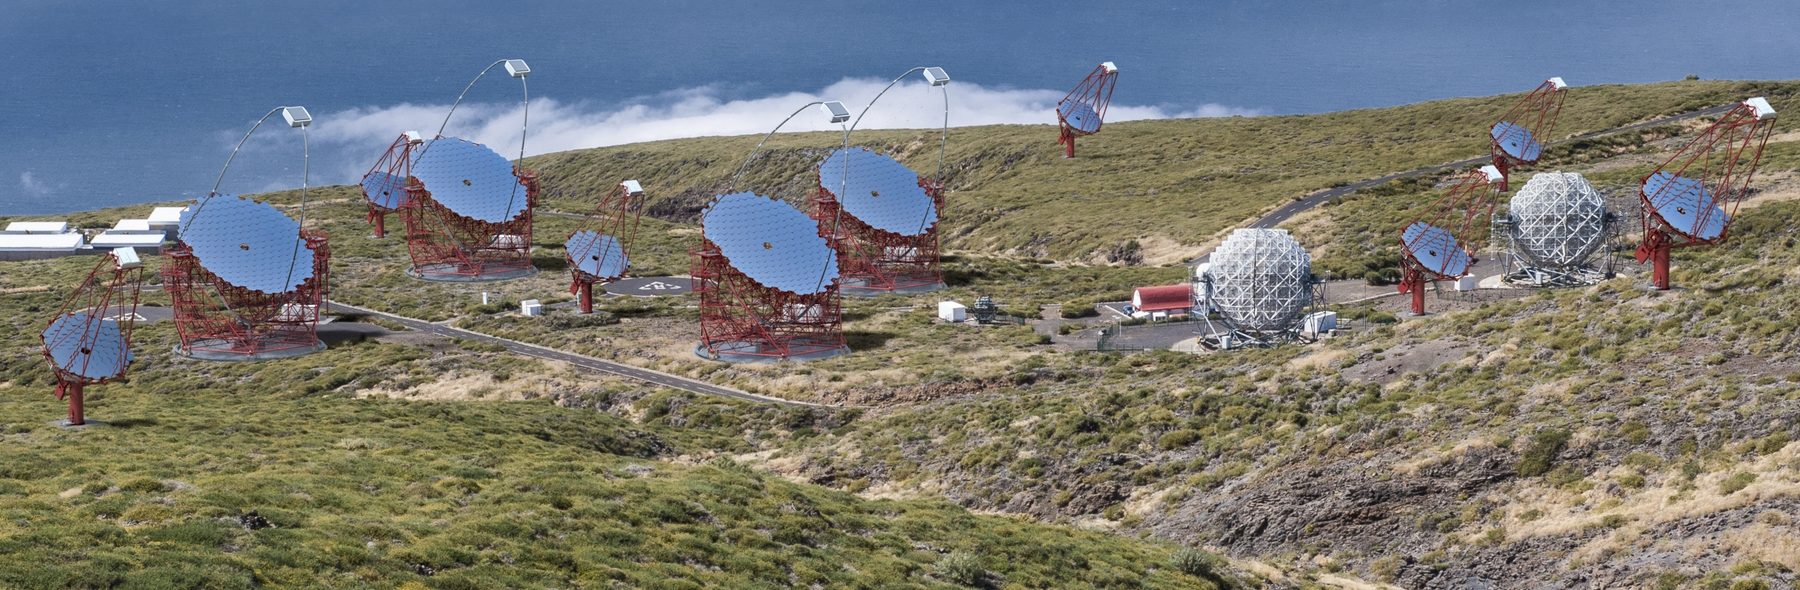
\includegraphics[width=\textwidth]{graphics/cta_north_render.jpg}
      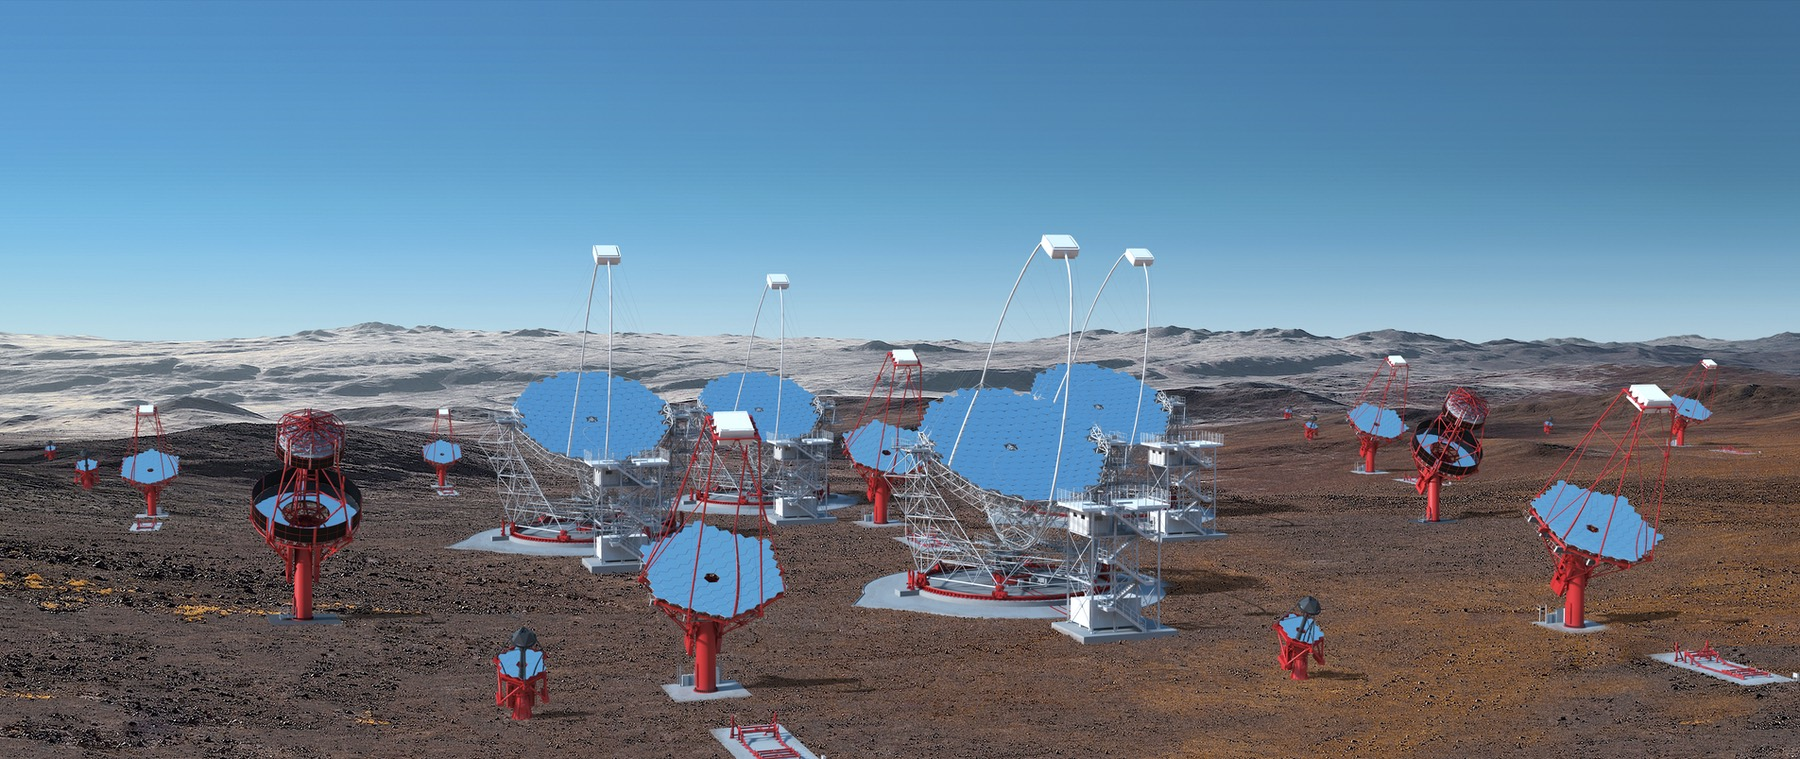
\includegraphics[width=\textwidth]{graphics/cta_south_render.jpg}
      \footcite{perezdiaz}
    \end{center}
  \end{minipage}
\end{frame}


\subsection{CTAs low-level data processing pipeline software: \texttt{ctapipe}}
\begin{frame}{\texttt{ctapipe}}
  \centering
  \ifdefined\darktheme
    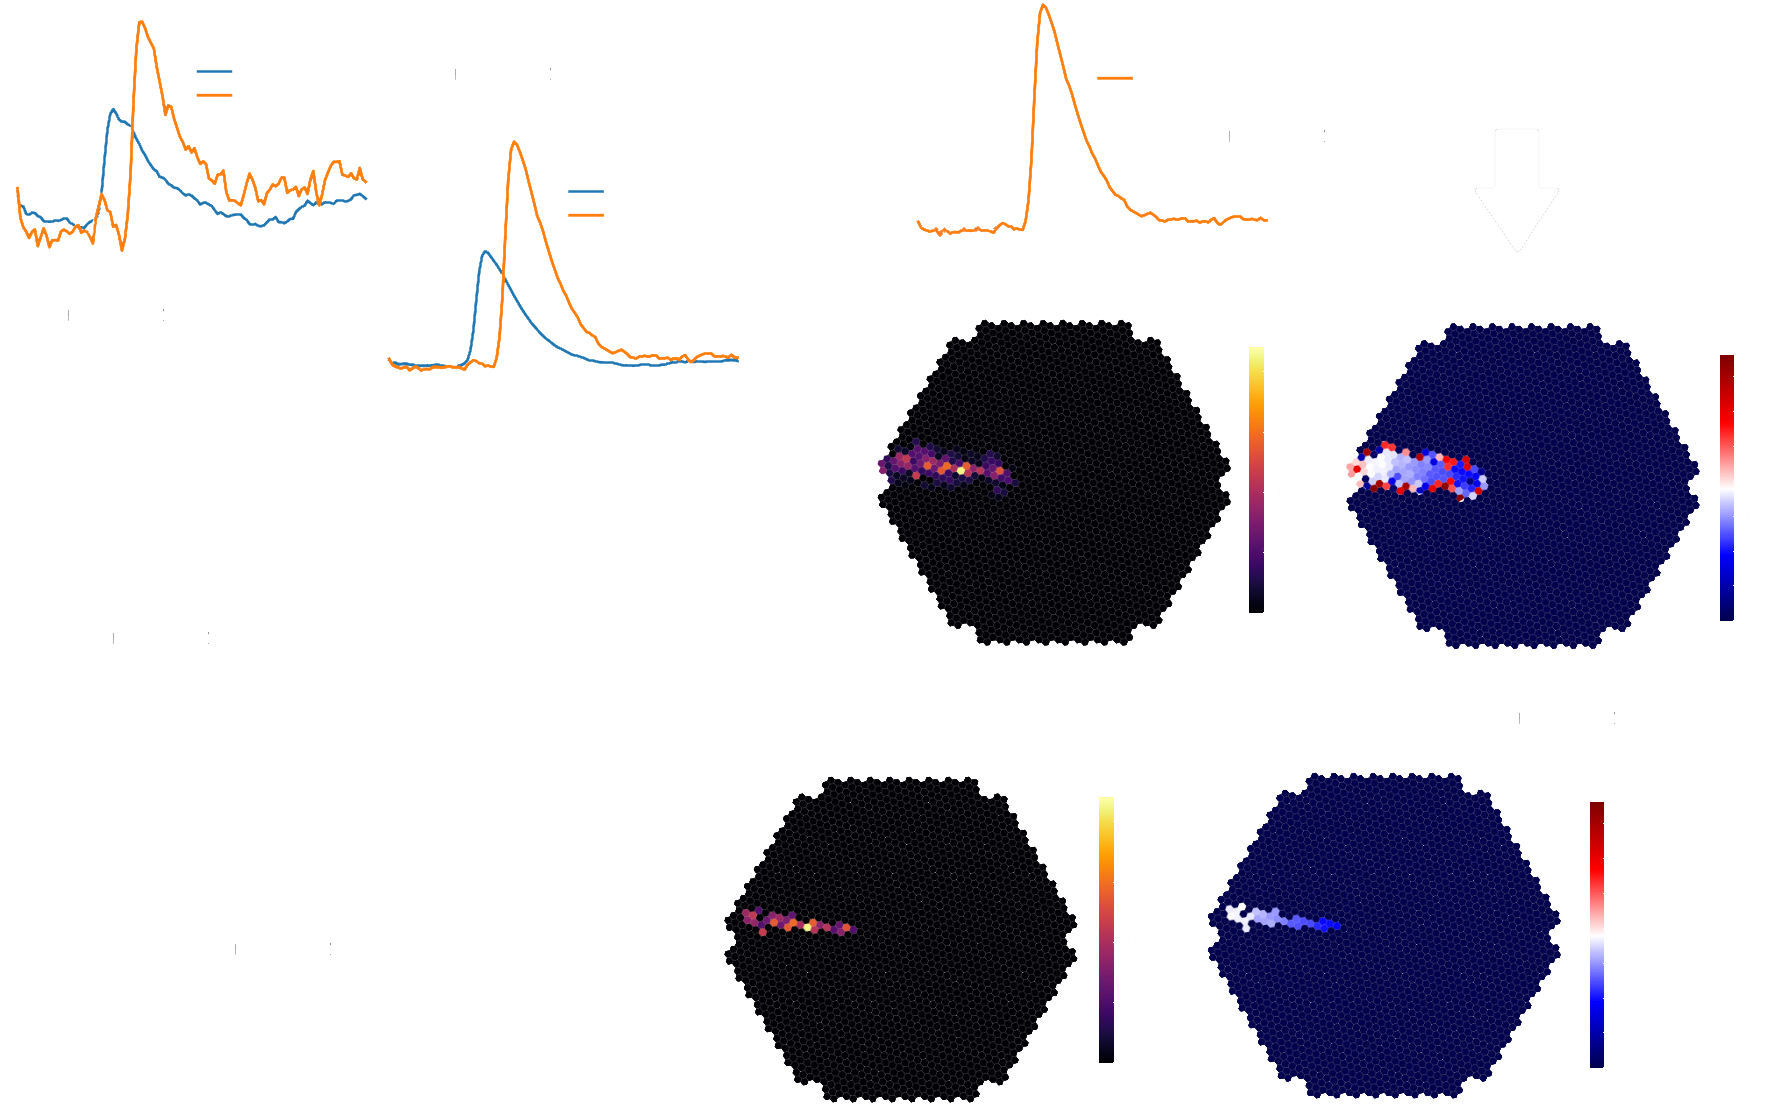
\includegraphics[width=0.7\textwidth]{graphics/ctapipe_darktheme.png}
    \footcite{hackfeld}
  \else
    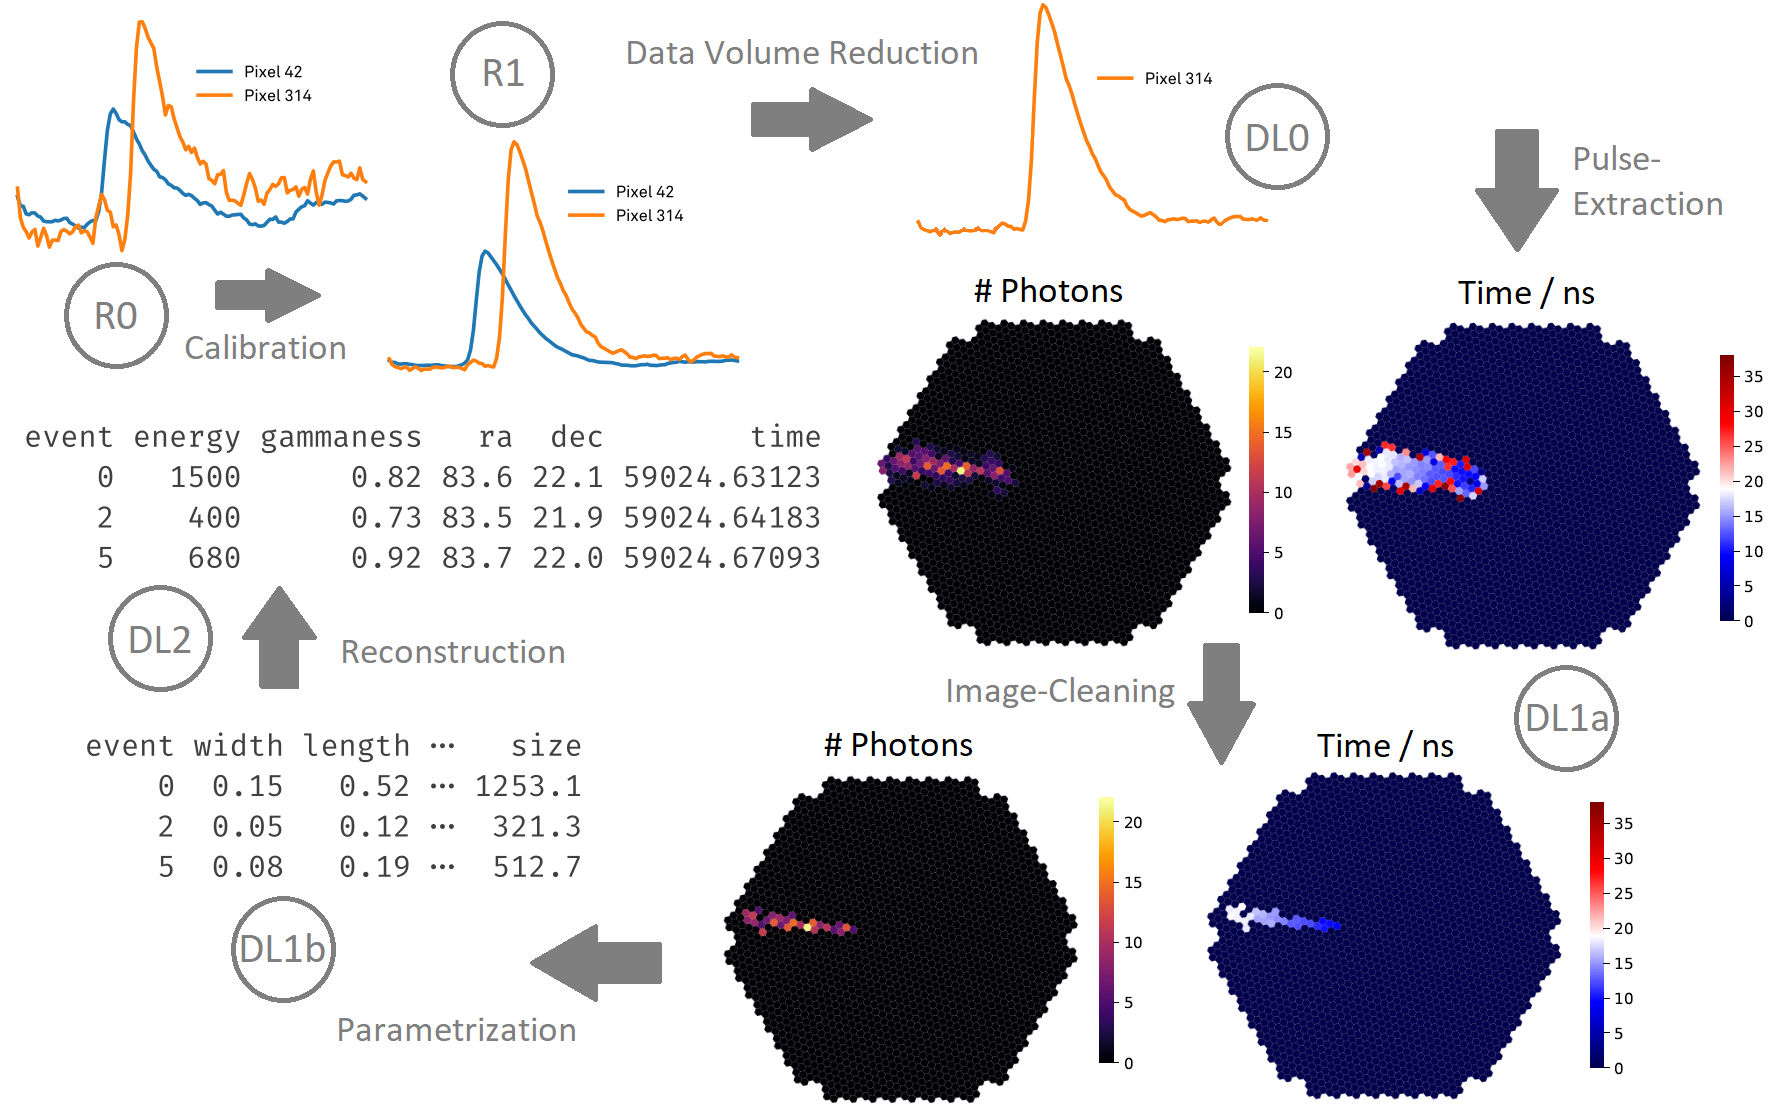
\includegraphics[width=0.7\textwidth]{graphics/ctapipe.png}
    \footcite{hackfeld}
  \fi
\end{frame}

\subsection{Cleaning Algorithms}
\ifdefined\darktheme
  \begin{frame}[t]{Cleaning Algorithms}
    \raisebox{10ex}{
    \begin{overlayarea}{0.36\textwidth}{3.5cm}
      \only<1>{
      \begin{itemize}
        \setlength\itemsep{1em}
        \item \code{white}{TailcutsImageCleaner}
        \item \code{white}{MARSImageCleaner}
        \item \code{white}{FACTImageCleaner}
        \item \code{white}{TimeConstrainedImageCleaner}
      \end{itemize}
      }
      \only<2>{
      \begin{itemize}
        \setlength\itemsep{1em}
        \item \code{white}{TailcutsImageCleaner}
        \item \code{white!50!black}{MARSImageCleaner}
        \item \code{white!50!black}{FACTImageCleaner}
        \item \code{white!50!black}{TimeConstrainedImageCleaner}
      \end{itemize}
      }
      \only<3>{
      \begin{itemize}
        \setlength\itemsep{1em}
        \item \code{white!50!black}{TailcutsImageCleaner}
        \item \code{white}{MARSImageCleaner}
        \item \code{white!50!black}{FACTImageCleaner}
        \item \code{white!50!black}{TimeConstrainedImageCleaner}
      \end{itemize}
      }
      \only<4>{
      \begin{itemize}
        \setlength\itemsep{1em}
        \item \code{white!50!black}{TailcutsImageCleaner}
        \item \code{white!50!black}{MARSImageCleaner}
        \item \code{white}{FACTImageCleaner}
        \item \code{white!50!black}{TimeConstrainedImageCleaner}
      \end{itemize}
      }
      \only<5>{
      \begin{itemize}
        \setlength\itemsep{1em}
        \item \code{white!50!black}{TailcutsImageCleaner}
        \item \code{white!50!black}{MARSImageCleaner}
        \item \code{white!50!black}{FACTImageCleaner}
        \item \code{white}{TimeConstrainedImageCleaner}
      \end{itemize}
      }
    \end{overlayarea}
    }
    \raisebox{10ex}{
    \begin{overlayarea}{0.58\textwidth}{3.5cm}
      \only<2>{
      \begin{itemize}%TailcutsImageCleaner
        \item [•] Selects pixels that pass a \code{white!70!black}{picture} and \code{white!70!black}{boundary threshold}
        \item [•] Most basic implementation of the cleaning algorithms
      \end{itemize}
      }
      \only<3>{
      \begin{itemize}%MARSImageCleaner
        \item [•] Selects pixels that pass a \code{white!70!black}{picture} and \code{white!70!black}{boundary threshold}, analogous to \code{white!70!black}{TailcutsImageCleaner}
        \item [•] Also selects pixels that are a neighbor of a neighbor of a core pixel, if they are above the \code{white!70!black}{boundary threshold}
      \end{itemize}
      }
      \only<4>{
      \begin{enumerate}%FACTImageCleaner
        \item Finds all pixels that contain more photons than the \code{white!70!black}{picture threshold}
        \item Removes pixels with less than \(N\) neighbors
        \item Adds remaining neighbors that are above the \code{white!70!black}{boundary threshold}
        \item Removes pixels that have less than \(N\) neighbors, that arrive within a given timeframe
        \item Removes pixels that have less than \(N\) neighbors
        \item Removes pixels that have less than \(N\) neighbors, arriving within a given timeframe
      \end{enumerate}
      }
      \only<5>{
      \begin{enumerate}%TimeConstrainedImageCleaner
        \item Finds all core pixels above the \code{white!70!black}{picture threshold}
        \item Removes pixels with less than \(N\) neighbors
        \item Removes all pixels that arrive within a time limit of the average arrival time
        \item Finds all neighbboring pixels above the \code{white!70!black}{boundary threshold}
        \item Removes all pixels with less than \(N\) neighbors arriving within a given timeframe
      \end{enumerate}
      }
    \end{overlayarea}
    }
    \only<2>{
      \centering
      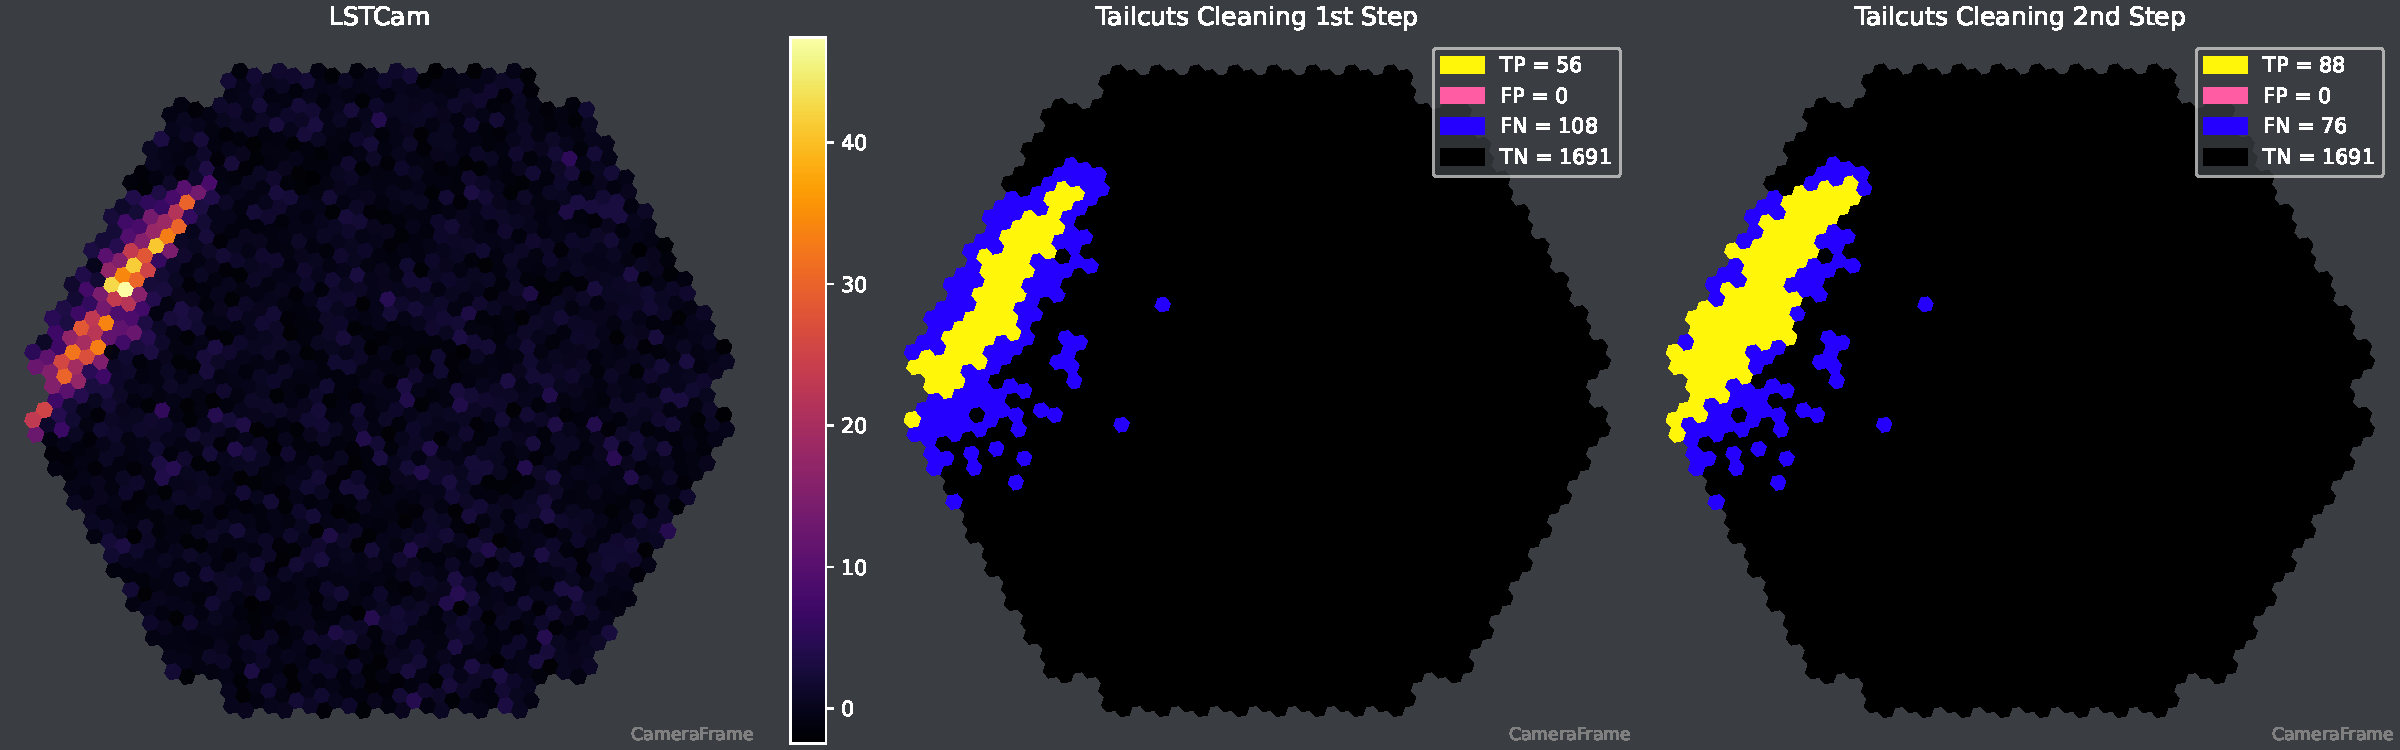
\includegraphics[height=0.15\textwidth]{plots/dl1_plots/run990_999_Tailcuts_event_463.pdf}
    }
    \only<3>{
      \centering
      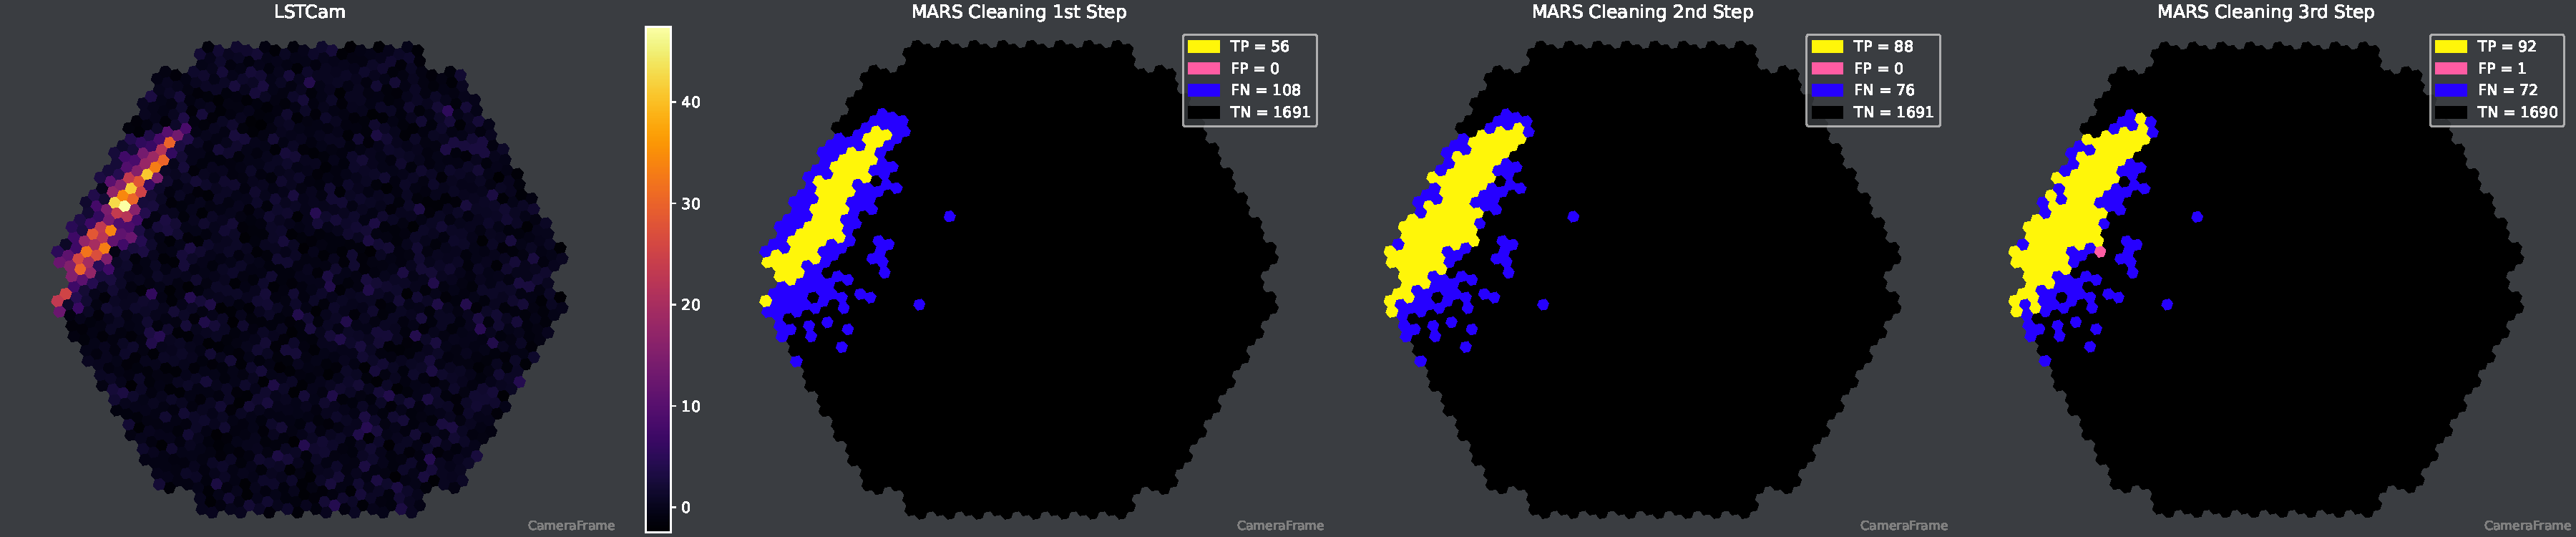
\includegraphics[height=0.15\textwidth]{plots/dl1_plots/run990_999_MARS_event_463.pdf}
    }
    \only<4>{
      \centering
      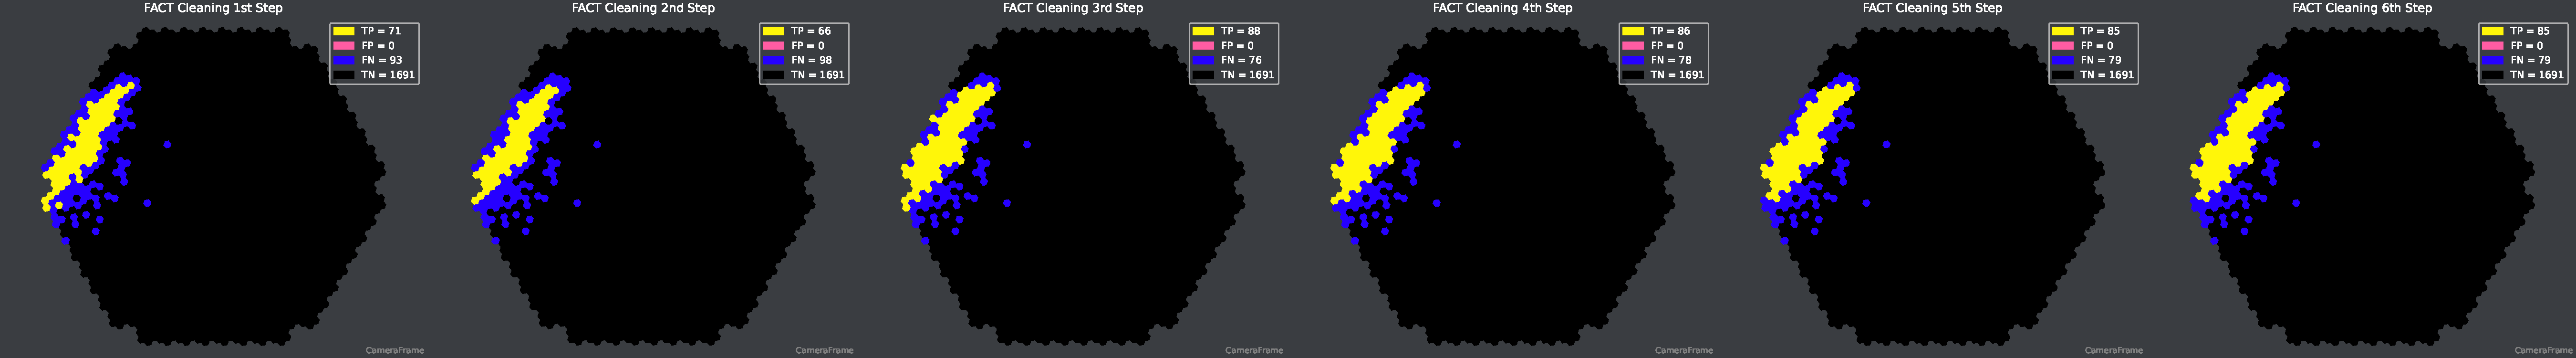
\includegraphics[height=0.13\textwidth]{plots/dl1_plots/run990_999_FACT_event_463.pdf}
    }
    \only<5>{
      \centering
      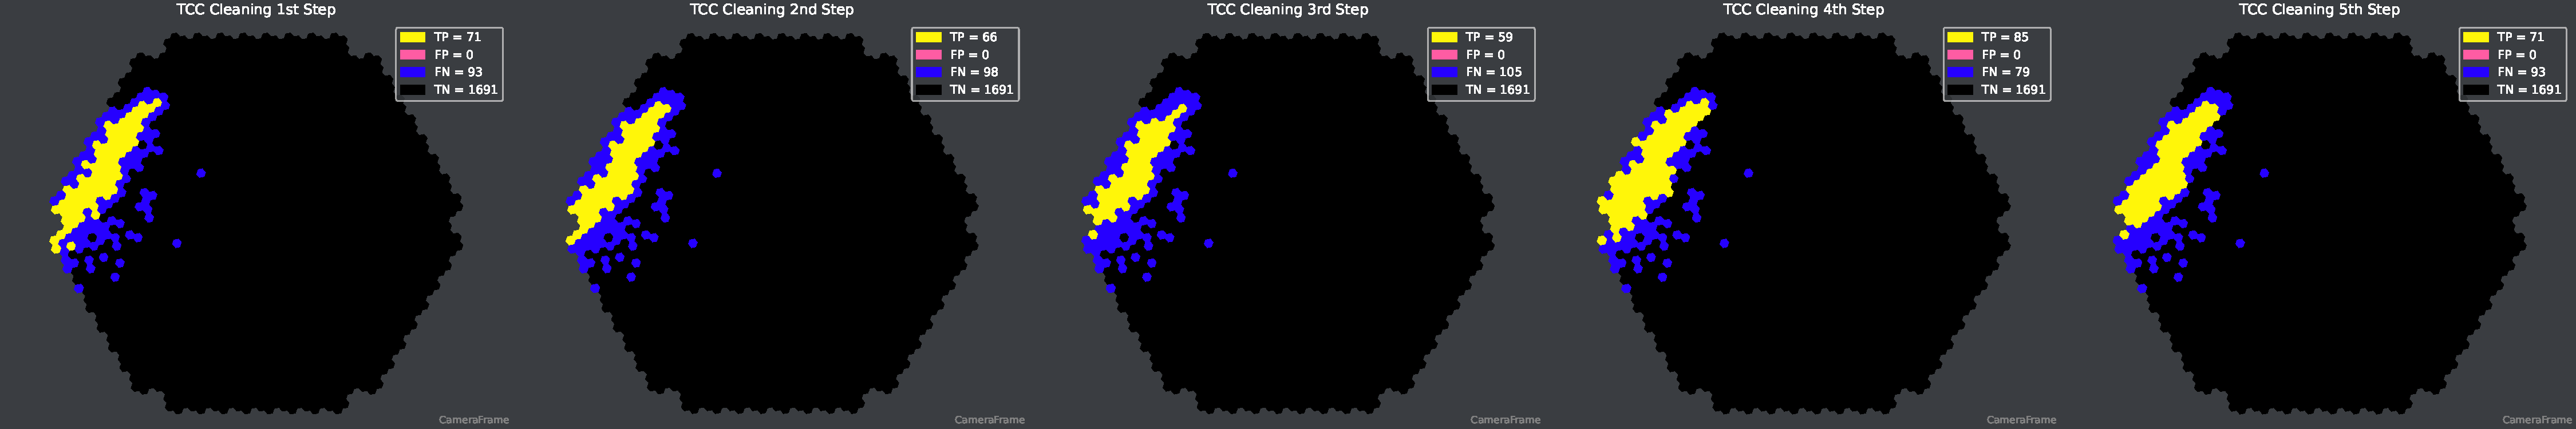
\includegraphics[height=0.15\textwidth]{plots/dl1_plots/run990_999_TCC_event_463.pdf}
    }
  \end{frame}
\else
  \begin{frame}{Cleaning Algorithms}
    \raisebox{10ex}{
    \begin{overlayarea}{0.36\textwidth}{3.5cm}
      \only<1>{
      \begin{itemize}
        \setlength\itemsep{1em}
        \item \code{darkgray}{TailcutsImageCleaner}
        \item \code{darkgray}{MARSImageCleaner}
        \item \code{darkgray}{FACTImageCleaner}
        \item \code{darkgray}{TimeConstrainedImageCleaner}
      \end{itemize}
      }
      \only<2>{
      \begin{itemize}
        \setlength\itemsep{1em}
        \item \code{darkgray}{TailcutsImageCleaner}
        \item \code{lightergray}{MARSImageCleaner}
        \item \code{lightergray}{FACTImageCleaner}
        \item \code{lightergray}{TimeConstrainedImageCleaner}
      \end{itemize}
      }
      \only<3>{
      \begin{itemize}
        \setlength\itemsep{1em}
        \item \code{lightergray}{TailcutsImageCleaner}
        \item \code{darkgray}{MARSImageCleaner}
        \item \code{lightergray}{FACTImageCleaner}
        \item \code{lightergray}{TimeConstrainedImageCleaner}
      \end{itemize}
      }
      \only<4>{
      \begin{itemize}
        \setlength\itemsep{1em}
        \item \code{lightergray}{TailcutsImageCleaner}
        \item \code{lightergray}{MARSImageCleaner}
        \item \code{darkgray}{FACTImageCleaner}
        \item \code{lightergray}{TimeConstrainedImageCleaner}
      \end{itemize}
      }
      \only<5>{
      \begin{itemize}
        \setlength\itemsep{1em}
        \item \code{lightergray}{TailcutsImageCleaner}
        \item \code{lightergray}{MARSImageCleaner}
        \item \code{lightergray}{FACTImageCleaner}
        \item \code{darkgray}{TimeConstrainedImageCleaner}
      \end{itemize}
      }
    \end{overlayarea}
    }
    \raisebox{10ex}{
    \begin{overlayarea}{0.58\textwidth}{3.5cm}
      \only<2>{
      \begin{itemize}%TailcutsImageCleaner
        \item [•] Selects pixels that pass a \code{lightgray}{picture} and \code{lightgray}{boundary threshold}
        \item [•] Most basic implementation of the cleaning algorithms
      \end{itemize}
      }
      \only<3>{
      \begin{itemize}%MARSImageCleaner
        \item [•] Selects pixels that pass a \code{lightgray}{picture} and \code{lightgray}{boundary threshold}, analogous to \code{lightgray}{TailcutsImageCleaner}
        \item [•] Also selects pixels that are a neighbor of a neighbor of a core pixel, if they are above the \code{lightgray}{boundary threshold}
      \end{itemize}
      }
      \only<4>{
      \begin{enumerate}%FACTImageCleaner
        \item Finds all pixels that contain more photons than the \code{lightgray}{picture threshold}
        \item Removes pixels with less than \(N\) neighbors
        \item Adds remaining neighbors that are above the \code{lightgray}{boundary threshold}
        \item Removes pixels that have less than \(N\) neighbors, that arrive within a given timeframe
        \item Removes pixels that have less than \(N\) neighbors
        \item Removes pixels that have less than \(N\) neighbors, arriving within a given timeframe
      \end{enumerate}
      }
      \only<5>{
      \begin{enumerate}%TimeConstrainedImageCleaner
        \item Finds all core pixels above the \code{lightgray}{picture threshold}
        \item Removes pixels with less than \(N\) neighbors
        \item Removes all pixels that arrive within a time limit of the average arrival time
        \item Finds all neighbboring pixels above the \code{lightgray}{boundary threshold}
        \item Removes all pixels with less than \(N\) neighbors arriving within a given timeframe
      \end{enumerate}
      }
    \end{overlayarea}
    }
    \only<2>{
      \centering
      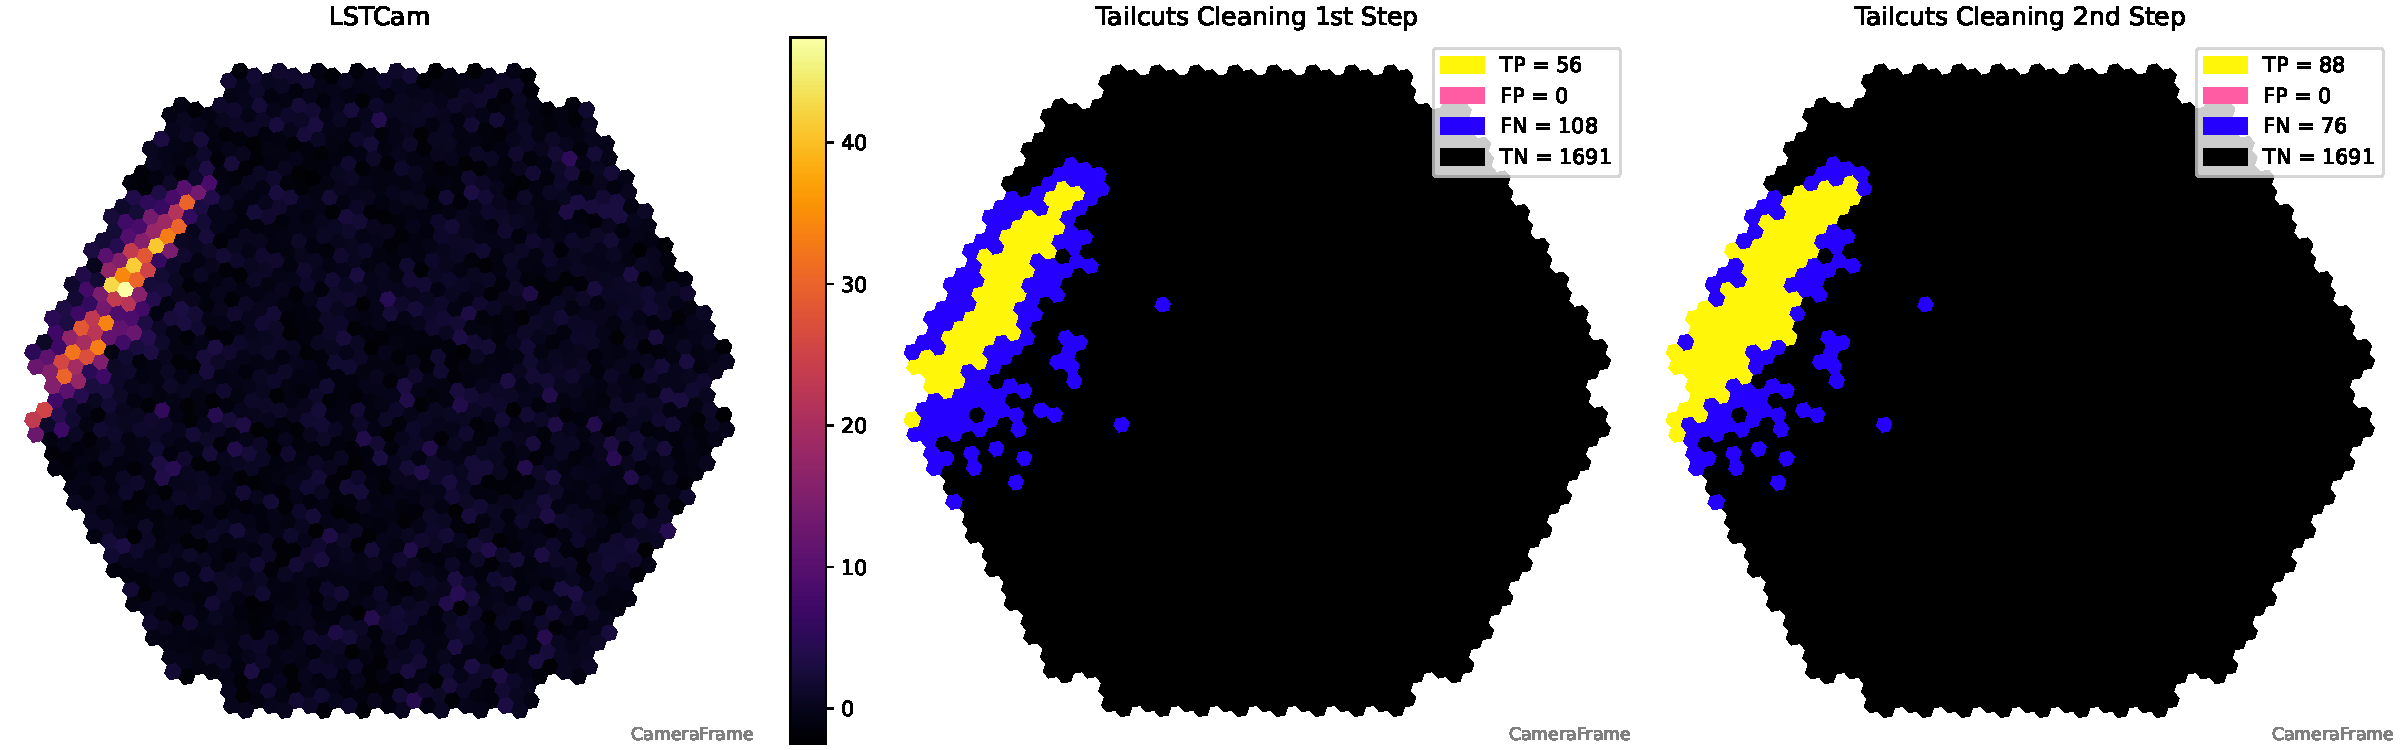
\includegraphics[height=0.15\textwidth]{plots/dl1_plots/run990_999_Tailcuts_event_463_light.pdf}
    }
    \only<3>{
      \centering
      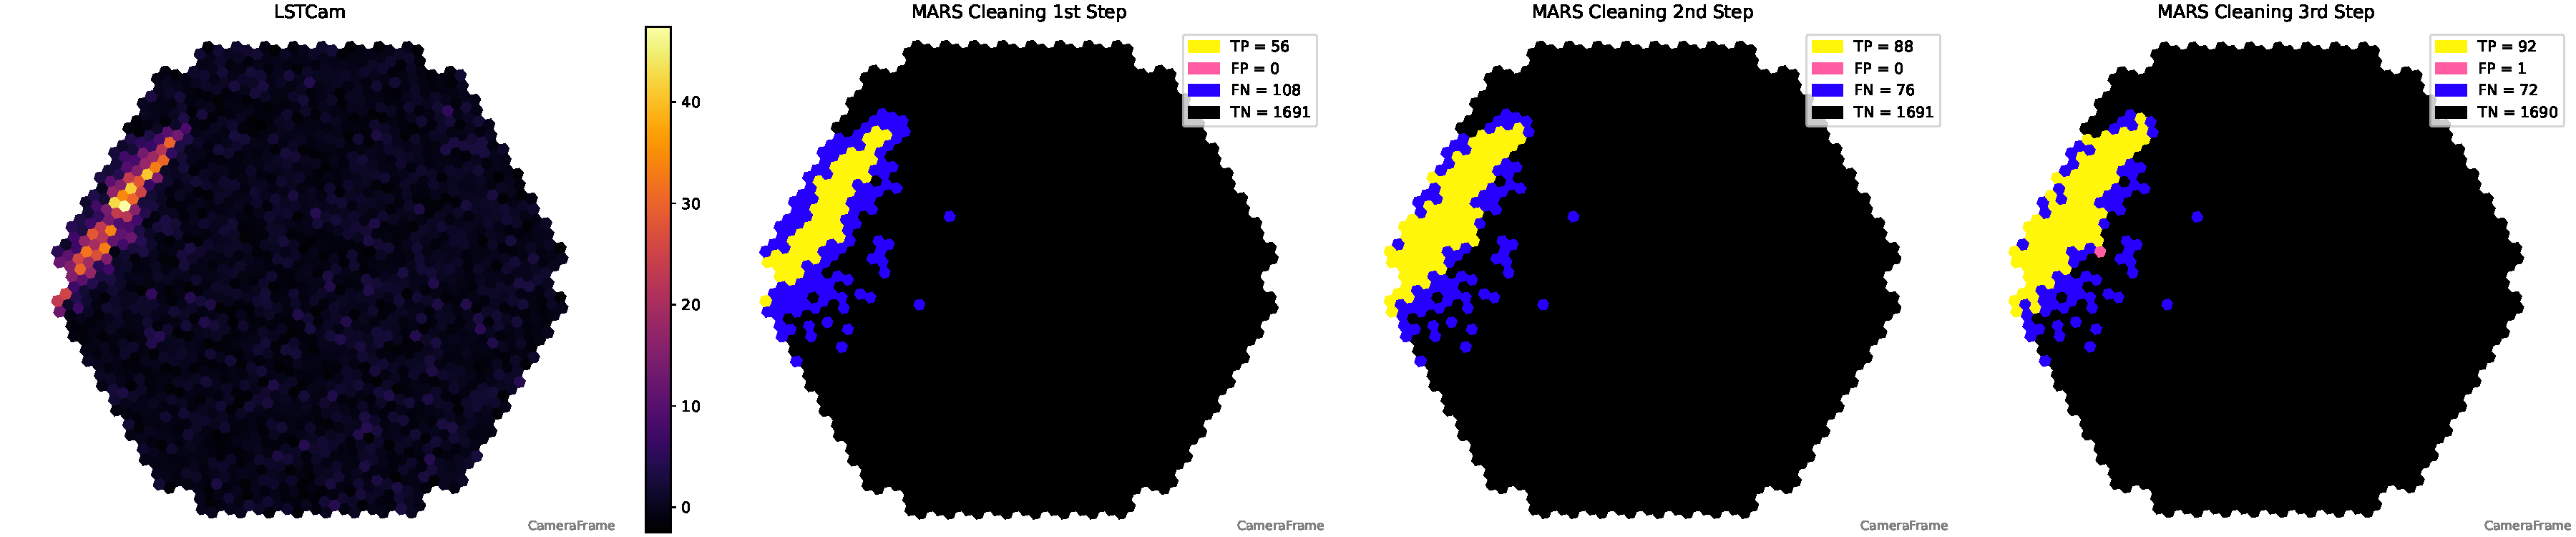
\includegraphics[height=0.15\textwidth]{plots/dl1_plots/run990_999_MARS_event_463_light.pdf}
    }
    \only<4>{
      \centering
      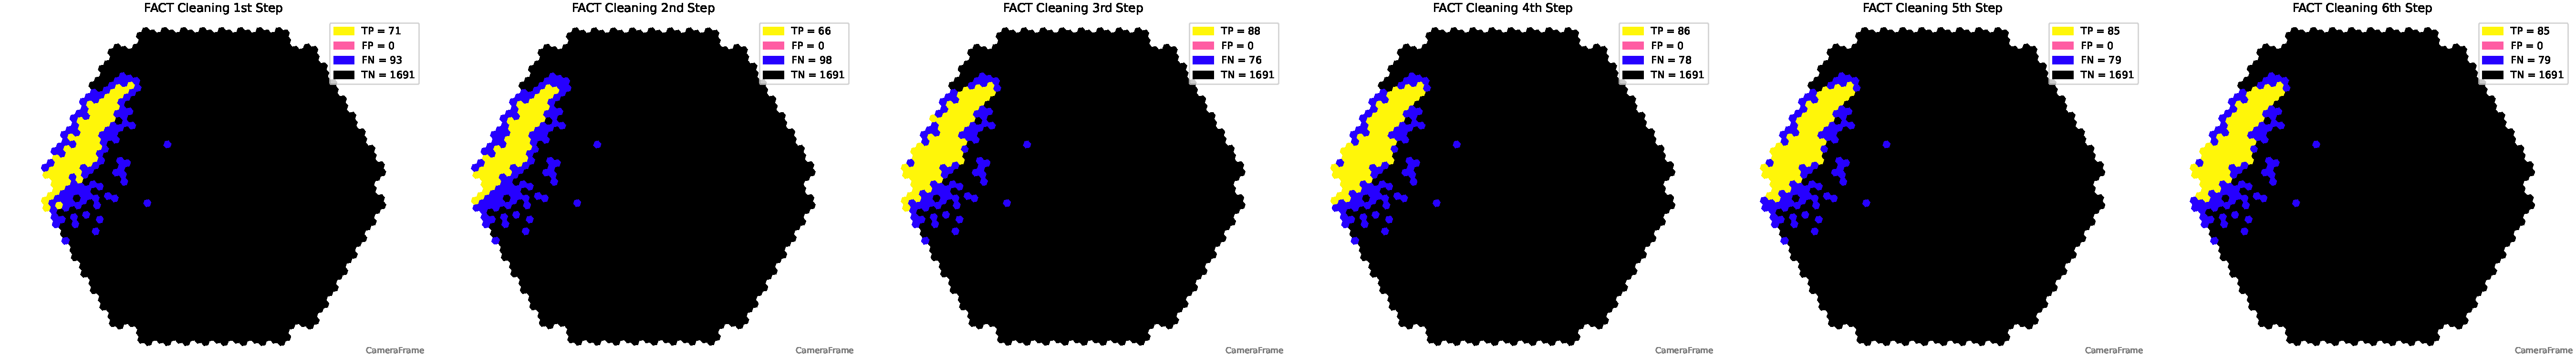
\includegraphics[height=0.13\textwidth]{plots/dl1_plots/run990_999_FACT_event_463_light.pdf}
    }
    \only<5>{
      \centering
      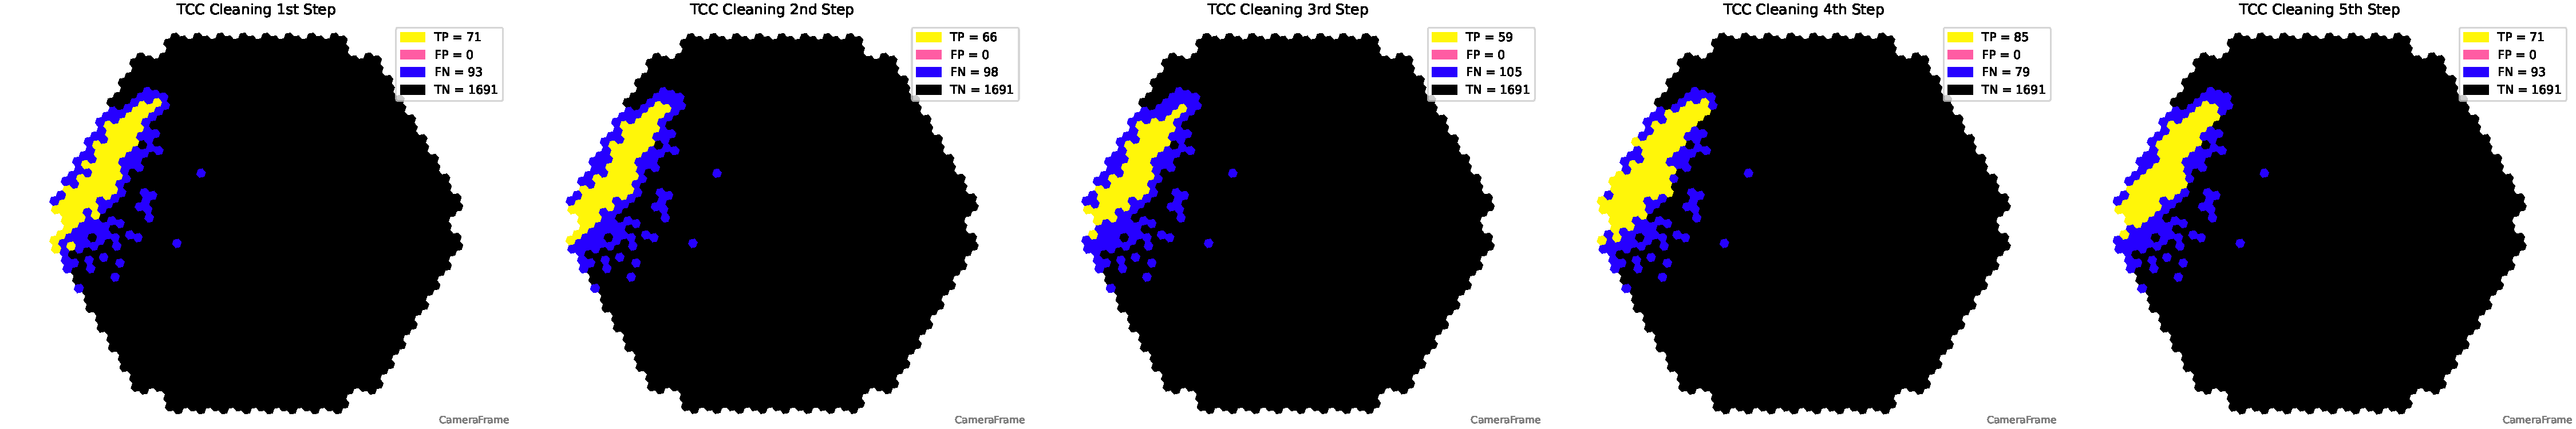
\includegraphics[height=0.15\textwidth]{plots/dl1_plots/run990_999_TCC_event_463_light.pdf}
    }
  \end{frame}
\fi